\documentclass{article}
\usepackage{titlesec}
\usepackage[utf8]{inputenc}
\usepackage[a4paper, total={6in, 9in}]{geometry}
\usepackage{fancyhdr}
\usepackage{graphicx} % Add the graphicx package
\usepackage{lipsum} % For placeholder text
\usepackage{tikz}
\usepackage{cite}
\usepackage{bm}
\usepackage{acronym}
\usepackage{amsmath,amssymb,amsfonts}
\usepackage{algorithmic}
\usepackage{graphicx}
\usepackage{caption}
\usepackage{subcaption}
\captionsetup{font=small, labelfont=bf}
\captionsetup[sub]{labelsep=period, subrefformat=brace}
\usepackage{tikz}
\usepackage{textcomp}
\usepackage{xcolor}
\usepackage[numbers]{natbib}
\bibliographystyle{ieeetrann}
\usepackage{subfig}
\usepackage{svg}
\usepackage{multirow}
\usepackage{pdfpages}
\usepackage{listings}
\usepackage{xcolor}

\definecolor{codegreen}{rgb}{0,0.6,0}
\definecolor{codegray}{rgb}{0.5,0.5,0.5}
\definecolor{codepurple}{rgb}{0.58,0,0.82}
\definecolor{backcolour}{rgb}{0.95,0.95,0.92}

\lstdefinestyle{mystyle}{
    backgroundcolor=\color{backcolour},   
    commentstyle=\color{codegreen},
    keywordstyle=\color{magenta},
    numberstyle=\tiny\color{codegray},
    stringstyle=\color{codepurple},
    basicstyle=\ttfamily\footnotesize,
    breakatwhitespace=false,         
    breaklines=true,                 
    captionpos=b,                    
    keepspaces=true,                 
    numbers=left,                    
    numbersep=5pt,                  
    showspaces=false,                
    showstringspaces=false,
    showtabs=false,                  
    tabsize=2
}

\usepackage[
backend=biber,
style=numeric,
sorting=none
]{biblatex}

\addbibresource{references.bib}

\title{Bibliography management: \texttt{biblatex} package}
\author{Share\LaTeX}
\date{23/03/2024}

\lstset{style=mystyle}

% Set up page headers and footers
\pagestyle{fancy}
\fancyhf{}
\rhead{ }
\lhead{Simulation Assignment: Eye Diagrams and Equalization}
\cfoot{\thepage}

% Redefine the abstract environment to be single column
\renewenvironment{abstract}
{\par\noindent\textbf{\abstractname}\ \ignorespaces}{\par}

% Redefine section format
\titleformat{\section}
{\normalfont\Large\bfseries}{\thesection}{1em}{}

\begin{document}
	
	% Cover Page
	\begin{titlepage}
		
		\centering
		\vspace*{0.5cm}
		
\includegraphics[width=5cm]{logo.png} % Replace with the path to your university logo
		\par\vspace{0.02cm}
		Department of Electronic \& Telecommunication Engineering
  
            University of Moratuwa, Sri Lanka.
		\par\vspace{4.5cm}
		{\LARGE\bfseries Simulation Assignment}\\{\LARGE Eye Diagrams and Equalization\par}
		\vspace{3.7cm}
		\begin{tabular}{c c}
			& \\
            210594J &   Senavirathne I.U.B\\
            210609M	&	Silva M.K.Y.U.N.\\
		\end{tabular}\\
		\vspace{1.5cm}
            {Submitted in partial fulfilment of the requirements for the module\par}
		{EN 2074 Communication Systems Engineering\par}
	
		\vspace{0.5cm}
		{\large 28/04/2024\par}
		\vfill
	\end{titlepage}

        \newpage
        \tableofcontents
	\newpage

        \section{Introduction}
        This report discusses and analyzes the performance of digital communication systems in various pulse-shaping methodologies and environments. Further, it explores the Impact of Additive White Gaussian Noise (AWGN) and Zero Forcing (ZF) Equalizer for multipath channels.\\

        \subsection{Pulse Amplitude Modulation (PAM)}
        Pulse Amplitude Modulation is a scheme in which a set of discrete amplitudes of a pulse train is chosen to represent a set of symbols made of bits in a bit stream.  \\

        In this assignment, we are simulating a baseband 2-PAM system, where the system contains two symbols +1 and -1, with each symbol representing a single bit (\(\log_2(2) = 1\)). This is similar to Binary Phase Shift Keying (BPSK), since both will result in a similar modulation.

        \begin{align*}
            0 &\rightarrow -1 \quad (180^\circ \text{ phase}) \\
            1 &\rightarrow +1 \quad (0^\circ \text{ phase})
        \end{align*}

        \subsection{Pulse Shaping}
        Digital signals are generally transmitted in a sequence of pulses. The shape of these pulses can change due to various reasons such as bandwidth limitations, frequency and noise. These pulses should be following the Nyquist's First Criterion.\\ 

        \textbf{Rectangular Pulses} have zero inter-symbol interference. However, in the frequency domain, this requires an infinite bandwidth. \textbf{Sinc pulses} which satisfy the Nyquist's Criterion are time unlimited. \\

        As a solution for these problems, a scheme of modulation with \textbf{Raised Cosine Pulses} can be used. These pulses are band-limited, and highly time limited. They compromise between the bandwidth and the inter-symbol interference (ISI). By controlling the roll-off factor of the pulse, we can control the excess bandwidth.

        \subsection{Eye Diagrams}
        Eye diagrams are a tool that is used to analyse communication systems, by superimposing multiple successive symbols. The resulting plot would resemble a human eye, giving it its name. An eye diagram can reveal the following information about a system.\cite{onsemi}
        \begin{itemize}
            \item \textbf{Eye height} - Noise immunity
            \item \textbf{Eye width} - Error free region
            \item \textbf{Time variation at zero crossing} - A measure of jitter/ time offset
            \item \textbf{Thickness at the peaks} - Peak deviation
        \end{itemize}

        \subsection{Channel Equalisation}
        The purpose of using equalisation schemes is to compensate for the frequency-dependent amplitude and phase deviations, introduced to the original signal by the channel. These impairments include Inter-symbol Interference (ISI), multipath fading, and noise. These impairments can result in symbol errors. This can be managed by the introduction of equalizers into the communication system.\\

        Equalizers change the frequency response of the channel, adjusting the amplitude and frequency of the signal. One of such equalizers that are being used in communication systems is known as the \textbf{Zero Forcing (ZF) Equaliser}, an equaliser which tries to apply the inverse of the frequency response of the channel onto the signal, which we will be using in this assignment.

        \section{Assignment}
        \subsection{Task I}
        \textit{Reqiuerment:\\
        In Task I, you are expected to generate eye diagrams for baseband 2-PAM signalling with different pulse shaping filters.
            \begin{enumerate}
                \item Generate an impulse train representing BPSK symbols.
                \item Obtain transmit signal by convolving the impulse train with a pulse shaping filter where the impulse response is a Sinc function.
                \item Generate the eye diagram of the transmit signal
                \item Repeat 1-3 for raised cosine pulse shaping filters with roll-off factors 0.5 and 1.
                \item Compare the robustness of the system to noise, sampling time and synchronization errors.
            \end{enumerate}
        }\\

        In this assignment, we have generated 1000-bit symbols, which have been mapped to -1 and +1 in a 2-PAM scheme, or to \(0^\circ\) and \(180^\circ\). Each symbol has been sampled 10 times, creating 10000 samples. Then this is convoluted with a Sinc pulse having 2000 samples. 

        \begin{figure}[!htb]
                \centering
                \begin{tikzpicture}
                    \node at (0.5,-0.2){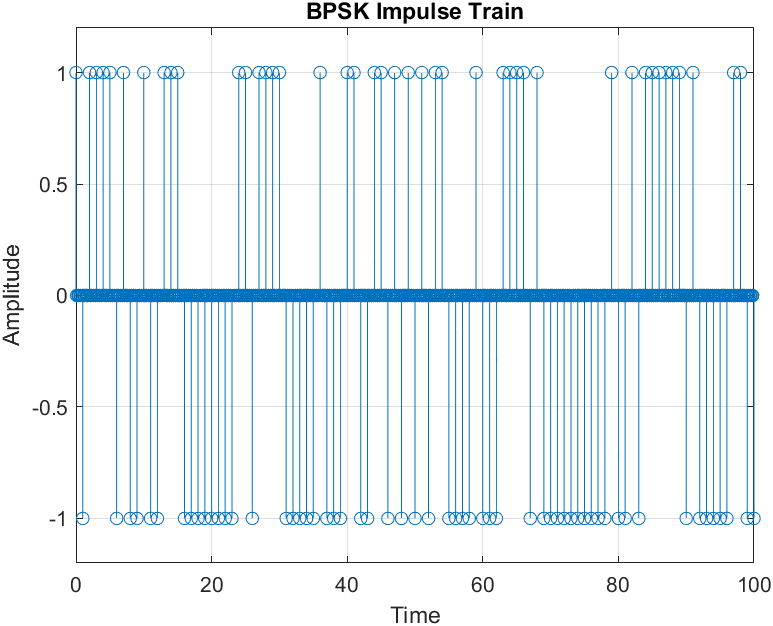
\includegraphics[width=10.5cm]{7.png}};
                \end{tikzpicture}
        \end{figure}
        
        \begin{figure}[!htb]
                \centering
                \begin{tikzpicture}
                    \node at (0.5,-0.2){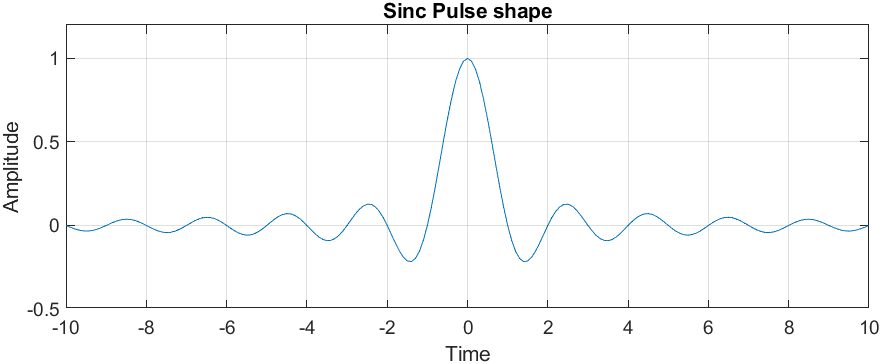
\includegraphics[width=10cm]{1.png}};
                \end{tikzpicture}
        \end{figure}

        Afterwards, these two were convoluted, and the following was obtained as the eye diagram of the resulting waveform.
        \begin{figure}[!htb]
                \centering
                \begin{tikzpicture}
                    \node at (0.5,-0.2){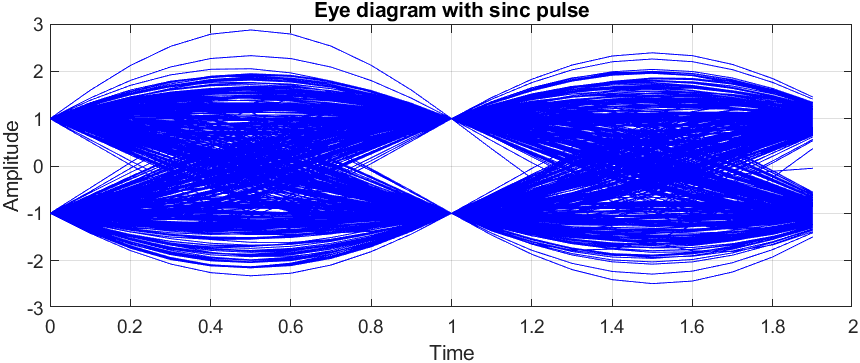
\includegraphics[width=10cm]{2.png}};
                \end{tikzpicture}
        \end{figure}

        Now the impulse train was convoluted with two \textbf{Raised Cosine} pulse shaping filters, each having a \textit{roll-off factor} of 0.5 and 1. The equation of a raised cosine pulse is as follows:\\

        \[h(t) = \begin{cases}
                \frac{\pi}{4T} \operatorname{sinc}\left(\frac{1}{2\beta}\right), & t = \pm \frac{T}{2\beta} \\
                \frac{1}{T} \operatorname{sinc}\left(\frac{t}{T}\right) \frac{\cos\left(\frac{\pi \beta t}{T}\right)}{1 - \left(\frac{2\beta t}{T}\right)^2}, & \text{otherwise}
            \end{cases}\]\\

        in which \(\beta\) is the Roll off factor, and \(T\) is the symbol period. In this assignment \(T=1\) has been used, and \(\beta = 0.5\) and \(\beta = 1\) which leads the following waveforms have been used.

        \begin{figure}[!htb]
                \centering
                \begin{tikzpicture}
                    \node at (0.5,-0.2){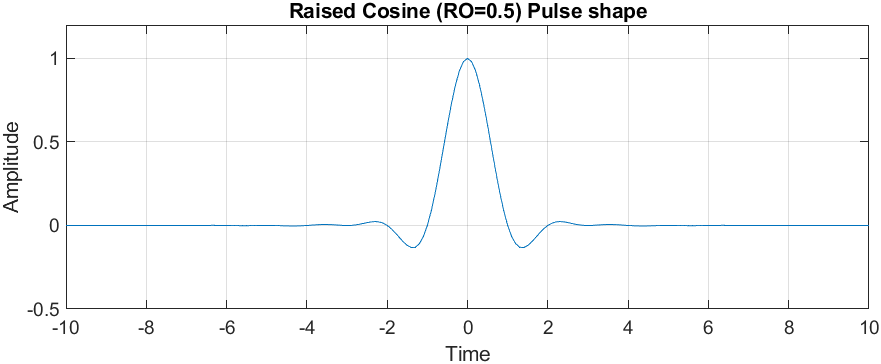
\includegraphics[width=10cm]{3.png}};
                \end{tikzpicture}
        \end{figure}

        \begin{figure}[!htb]
                \centering
                \begin{tikzpicture}
                    \node at (0.5,-0.2){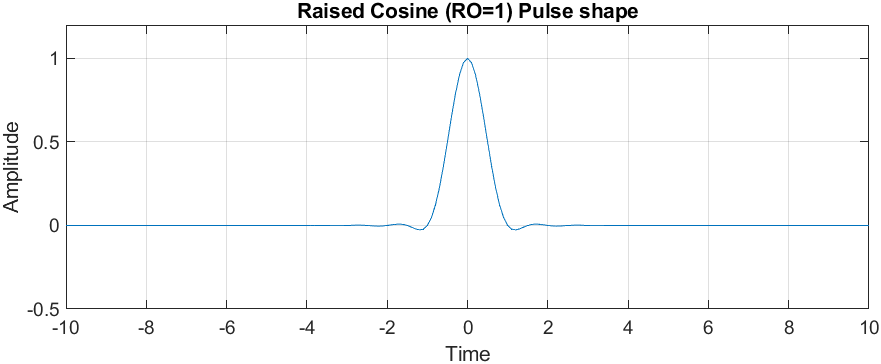
\includegraphics[width=10cm]{5.png}};
                \end{tikzpicture}
        \end{figure}

        \newpage
        When the impulse train is convoluted with the above waveforms, it leads with the following eye diagrams.

        \begin{figure}[!htb]
                \centering
                \begin{tikzpicture}
                    \node at (0.5,-0.2){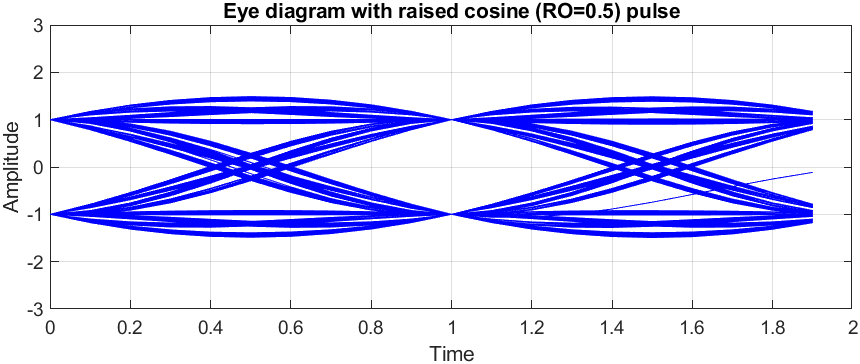
\includegraphics[width=10cm]{4.png}};
                \end{tikzpicture}
        \end{figure}

        \begin{figure}[!htb]
                \centering
                \begin{tikzpicture}
                    \node at (0.5,-0.2){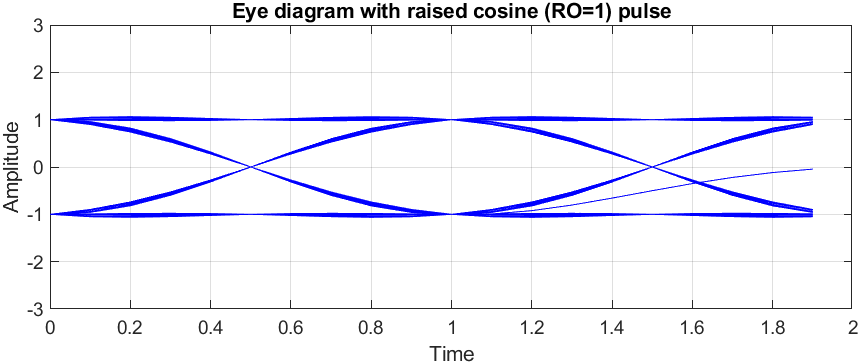
\includegraphics[width=10cm]{6.png}};
                \end{tikzpicture}
        \end{figure}

        By the above eye diagrams, we can arrive at some conclusions:
        \begin{itemize}
            \item Eye width in the increasing order can be seen in the sinc, raised cosine of rollover 0.5 and 1. This implies that in the sinc pulse modulation, there is the least range for error-free sampling, with raised cosines of rollover 0.5 and 1 having more range in the increasing order
            \item Time variation at the zero crossing decreases from sinc to raised cosine of rollover 0.5 to 1, signifying decreasing time jitter. 0.5 rollover scheme has almost no jitter at all.
        \end{itemize} 

        By the above conclusion, we can predict that the sinc pulse, raised cosine with 0.5 roll-over, and 1 rollover will predict better in a noisy channel, in the increasing order. 

        \newpage
        \subsection{Task II}
        \textit{Requirement:\\
        In Task 2, you are required to repeat Task 1, in the presence of additive white Gaussian noise (AWGN). To generate noise, use \texttt{randn} function. Set the variance of noise such that \(\frac{E_b}{N_0} = 10 dB\), where \(E_b\) is the average bit energy and \(N_0\) is the noise power spectral density.}\\

        Here Additive White Gaussian Noise (AWGN) has a mean of 0 and a variance such that \(\frac{E_b}{N_0} = 10 dB\), where \(E_b\) is the average bit energy and \(N_0\) is the noise power spectral density is added to the output of the filter. This leads to the following eye diagrams:

        \begin{figure}[!htb]
                \centering
                \begin{tikzpicture}
                    \node at (0.5,-0.2){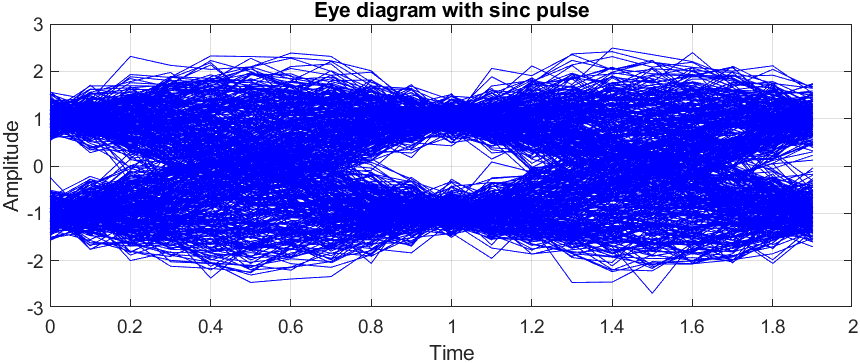
\includegraphics[width=10cm]{9.png}};
                \end{tikzpicture}
        \end{figure}

        \begin{figure}[!htb]
                \centering
                \begin{tikzpicture}
                    \node at (0.5,-0.2){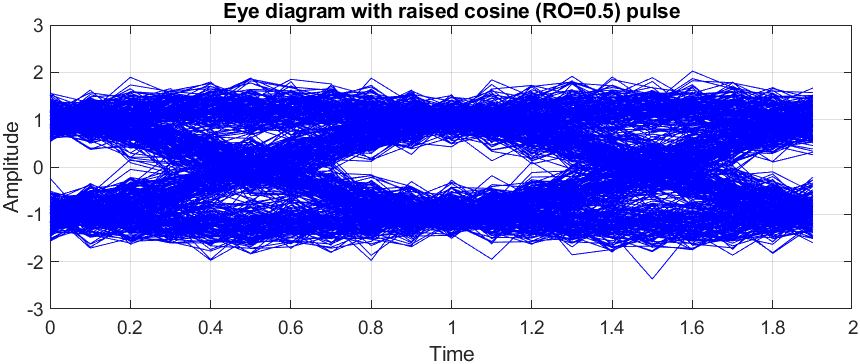
\includegraphics[width=10cm]{10.png}};
                \end{tikzpicture}
        \end{figure}

        \begin{figure}[!htb]
                \centering
                \begin{tikzpicture}
                    \node at (0.5,-0.2){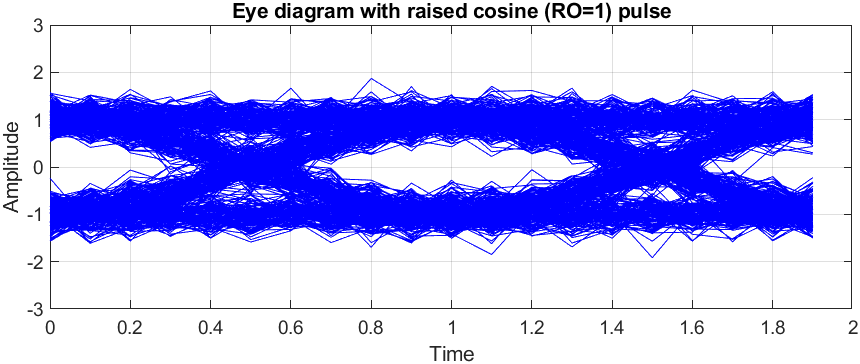
\includegraphics[width=10cm]{11.png}};
                \end{tikzpicture}
        \end{figure}

        From the above eye diagrams, we can arrive at some conclusions:
        \begin{itemize}
            \item We can see the eye heights of all three diagrams have reduced due to the addition of AWGN. However, the eye height increases from sinc pulse to raised cosines with the rollover of 0.5 and to that of 1. This signifies the increasing noise immunity.
            \item Due to the new AWGN, the eye widths have reduced, but still are in increasing order, as can be seen in the sinc, raised cosine of rollover 0.5 and 1. This implies that in the sinc pulse modulation, there is the least range for error-free sampling, with raised cosines of rollover 0.5 and 1 having more range in the increasing order
            \item Time variation at the zero crossing has increased, but still decreased from sinc to raised cosine of rollover 0.5 to 1, signifying decreasing time jitter. In this scenario, however, a scheme with a rollover of 1 is not devoid of jitter. 
            \item Here in the presence of noise, there is a thickness at the peak of the eye diagram. This is due to the noise and may cause some errors in sampling.
        \end{itemize} 

        By the above conclusion, we can predict that the sinc pulse, raised cosine with 0.5 roll-over, and 1 rollover will predict better in a noisy channel, in the increasing order. \\\\\\

        \subsection{Task III}
        \textit{Requirement:\\
        For Task 3, you will design a zero-forcing (ZF) equalizer for a 3-tap multipath channel. Please follow the following steps for Task 3.}
        \textit{
            \begin{enumerate}
                \item Generate a random binary sequence.
                \item 2-PAM modulation - bit 0 represented as -1 and bit 1 represented as +1. You can ignore pulse shaping here. Assume you are transmitting impulses.
                \item Generate the received signal samples by convolving the symbols with a 3-tap multipath channel with impulse response \texttt{h = [0.3 0.7 0.4]}.
                \item Add White Gaussian noise such that \(\frac{E_b}{N_0} = 0 dB\).
                \item Computing the ZF equalization filters at the receiver for 3, 5, 7, and 9 taps in length.
                \item Demodulation and conversion to bits
                \item Calculate the bit error rate (BER) by counting the number of bit errors.
                \item Repeat steps 1-7 for \(\frac{E_b}{N_0}\) values \(0\)-\(10 dB\).
                \item Plot the BER for all tap settings and \(\frac{E_b}{N_0}\) values in the same figure.
                \item Plot the BER for an additive white Gaussian noise (AWGN) channel in the same figure.
                \item Why there is a discrepancy between the AWGN channel BER and the ZF equalized multipath channel. Explain your results referring to the design of the ZF equalizer.
                \item Comment on the BER performance if binary orthogonal signalling was used instead of BPSK.
            \end{enumerate}
        }

        \newpage
        In this task we aim to revert the effects added onto a signal by a multipath channel, using a ZF equalizer. As an input for this, first, a binary sequence has been generated. Then this sequence has been modulated using a 2-PAM scheme, or BPSK scheme, mapping 0 to -1 and 1 to +1. Here we have not introduced a pulse shaping scheme as instructed.\\

        We have then simulated a multipath channel by convolving the transmitted signals with a \textit{3-tap impulse response}, represented by \texttt{h = [0.3, 0.9, 0.4]}, which would introduce inter-symbol interference. The multipath channel creates a signal using the shifted and weighed original signal.\\

        Afterwards, AWGN has been added to simulate a realistic environment. At first \(\frac{E_b}{N_0}\) is set to \(0 dB\). At the receiver, to combat the ISI, ZF filters at different tap lengths were made. Then this equalized signal is demodulated and then converted back into a bit stream. Calculating the Bit Error Rate (BER), we got the following for each tap:

        \begin{itemize}
            \item BER at 3 = 0.236783
            \item BER at 5 = 0.263130
            \item BER at 7 = 0.270090
            \item BER at 9 = 0.273533
        \end{itemize}

        Now these steps are repeated, with varying \(\frac{E_b}{N_0}\) values \(0\)-\(10 dB\). This leads to the following graph of bit error rate with the increasing \(\frac{E_b}{N_0}\):

        \begin{figure}[!htb]
                \centering
                \begin{tikzpicture}
                    \node at (0.5,-0.2){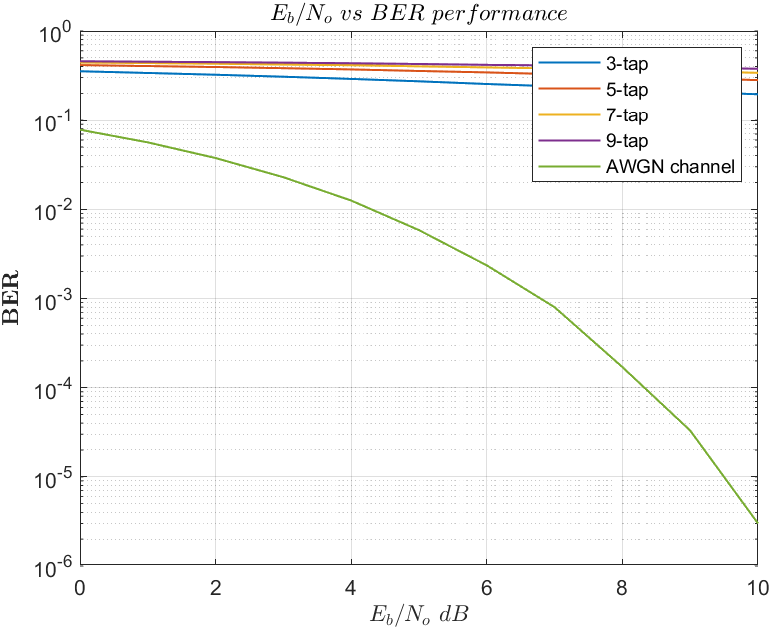
\includegraphics[width=10cm]{12.png}};
                \end{tikzpicture}
        \end{figure}

        In the AWGN channel, BER is very small compared to the ISI multipath channel with the ZF equalizer. The reason for this is the amplification of the noise at some frequency ranges by the ZF equalizer.\cite{art2}\\

        Further, any imperfect channel estimations may lead to higher BER. Also, rather than forcing the pulses to be zero at all the instances, we select a finite number of instances to tap. The residual interference of this will also contribute to performance issues.\cite{art3}\\

        \newpage
        Now let's consider the usage of binary orthogonal signalling, rather than BPSK. Here the distance between signals is smaller, as in BPSK it would have \(2\sqrt{E}\) and binary orthogonal would have \(\sqrt{2E}\) of a distance between the two symbols. Due to this, it will have a higher bit error rate than BPSK, in a given environment.\cite{art1}

        \begin{figure}[!htb]
                \centering
                \begin{tikzpicture}
                    \node at (0.5,-0.2){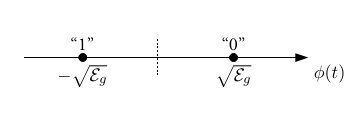
\includegraphics[width=5cm]{a.png}};
                \end{tikzpicture}
                \caption {Signal Constellation for BPSK}
        \end{figure}

        \begin{figure}[!htb]
                \centering
                \begin{tikzpicture}
                    \node at (0.5,-0.2){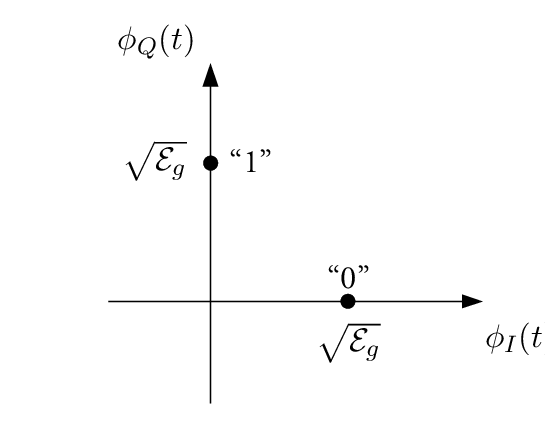
\includegraphics[width=5cm]{b.png}};
                \end{tikzpicture}
                \caption{Signal Constellation for Binary Orthogonal Signalling}
        \end{figure}

        \begin{figure}[!htb]
                \centering
                \begin{tikzpicture}
                    \node at (0.5,-0.2){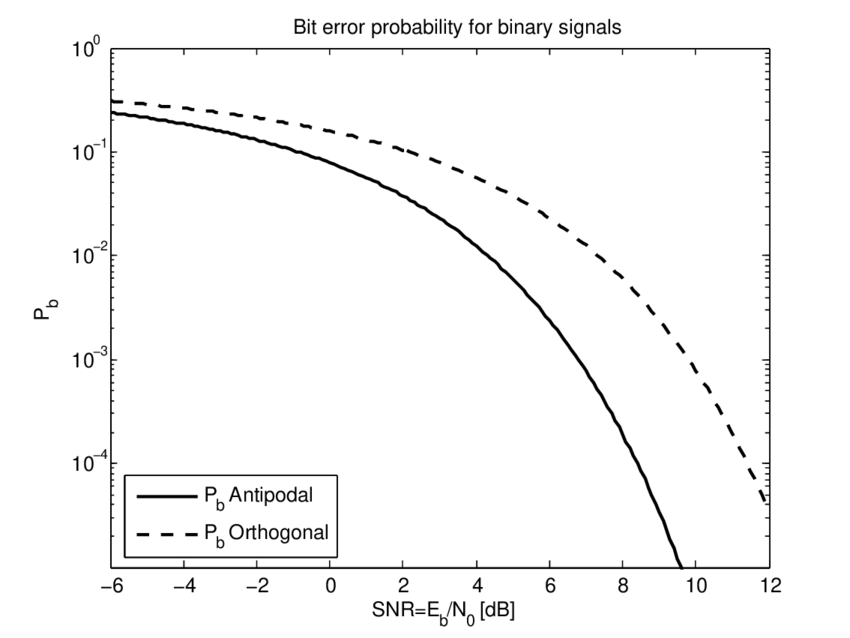
\includegraphics[width=10cm]{c.png}};
                \end{tikzpicture}
                \caption{BPSK vs Binary orthogonal BER performance}
        \end{figure}

        \newpage
        \printbibliography

        \newpage
        \section{Appendices}
        \subsection{Code for Task I}
        \lstinputlisting[language=Octave]{task1.m}

        \newpage
        \subsection{Code for Task II}
        \lstinputlisting[language=Octave]{task2.m}

        \newpage
        \subsection{Code for Task III}
        \lstinputlisting[language=Octave]{task3.m}        
\end{document}